\documentclass[a4paper]{article}

%% Language and font encodings
\usepackage[english]{babel}
\usepackage[utf8]{inputenc}
\usepackage[T1]{fontenc}

%% Sets page size and margins
\usepackage[a4paper,top=3cm,bottom=2cm,left=3cm,right=3cm,marginparwidth=1.75cm]{geometry}

%% Useful packages
\usepackage{float}
\usepackage{amsmath}
\usepackage{graphicx}
\usepackage[colorinlistoftodos]{todonotes}
\usepackage[colorlinks=true, allcolors=blue]{hyperref}

\title{Reporte de Actividad 3}
\author{Jonás Valenzuela Terán}

\begin{document}
\maketitle


\section*{Introducción}

La vida humana se encuentra casi totalmente encapsulada en la atmósfera, en la troposfera siendo específicos, aquí ocurren la mayor parte de los fenómenos meteorológicos, que influyen en gran manera a nuestras actividades personales y económicas, lo que da importancia al estudio del estado de la atmósfera y sus propiedades.

Se explicará a continuación que datos se recolectan, y como se usaron para analizarlos y obtener información, útil para pronósticos y precaución de peligros.

\section*{Fundamentos}

De las diferentes capas de la tierra, en la troposfera ocurren la mayor parte de los fenómenos meteorológicos, por lo que es estudiada con más detalle, utilizando sondeos atmosféricos.

Los sondeos atmosféricos realizan mediciones de distribuciones verticales de alguna propiedad física, tales como la presión, temperatura, contaminación, velocidad de vientos, concentración de ozono, etc...

El método más común es el llamado "globo del clima", que utiliza ondas microondas y infrarojo, y lleva todo el equipo necesario para tomar mediciones de propiedades físicas, registrando la ubicación exacta.

Estos datos pueden ser utilizados para realizar predicciones de clima numéricas, que toman los datos mencionados, y utilizando modelos matemáticos, predicen un estado futuro del clima, aunque solo fue posible hasta la disponibilidad de simulación super computadoras, y aun sigue siendo un reto por la naturaleza caótica de la atmósfera.



\section*{Análisis de Datos}

Recuperamos los datos de Sondeos Atmosféricos de la Universidad de Wyoming, se captaron datos de 1 solo sondeo, del 22 de diciembre y del 22 de junio, se eligió una ubicación central de la Antártida.

Para realizar el análisis, se leyeron los datos a través del entorno de programación Jupyter, con lenguaje de programación Python, para evitar problemas en la lectura, no se realizó lectura de las primeras 10 lineas, que contenían títulos, información textual de los datos, y muestras de datos incompletos.

Una vez realizado esto, se crearon gráficas de diferentes características meteorológicas de la ubicación, con respecto a la altura, para poder apreciar su comportamiento y compararlo en los tiempos diferentes de medición.

\section*{Resultados}

En general, se observa un clima mas estable en el mes de junio que en el mes de diciembre, a continuación se muestran las gráficas obtenidas de los datos.

En la figura 1, observamos que la presión tiene un comportamiento similar en ambos meses, con respecto a la altura. Observamos en la figura 2 que la temperatura si cambia su comportamiento, teniendo cambios más agresivos en diciembre. En las gráficas de la figura 3, se nota que la temperatura y temperatura de rocio se comportan de manera similar, solo variando en magnitud, pero con una variación más pronunciada en diciembre. Se distingue una gran diferencia entre la rapidez de vientos en junio y en diciembre en la figura 4, donde en junio la rapidez es mayormente uniforme, a diferencia de diciembre que varía significativamente. Finalmente, en la figura 5, se observa lo contrario, el mes de diciembre cuenta con una humedad relativa con una distribución más definida, en cambio, junio cuenta con variaciones con poco patrón.

\begin{figure}[h]
\begin{tabular}{ll}
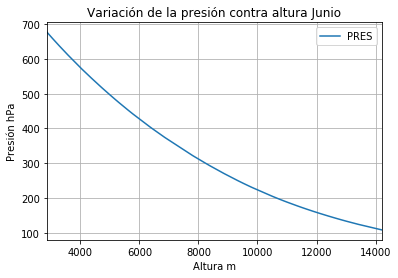
\includegraphics[scale=0.5]{grafica1.png}
&
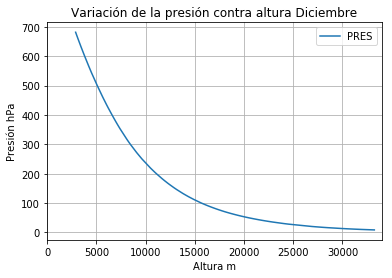
\includegraphics[scale=0.5]{grafica2.png}
\end{tabular}
\caption{Gráficas de variación de la presión contra altura}

\end{figure}


\begin{figure}[h]
\begin{tabular}{ll}
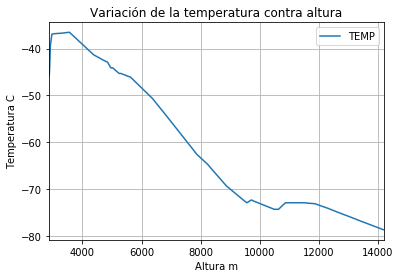
\includegraphics[scale=0.5]{grafica3.png}
&
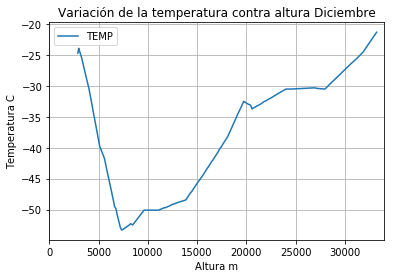
\includegraphics[scale=0.5]{grafica4.png}
\end{tabular}
\caption{Gráficas de variación de la temperatura contra altura}

\end{figure}


\begin{figure}[h]
\begin{tabular}{ll}
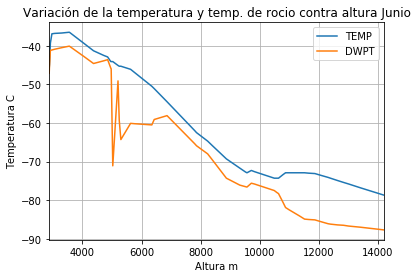
\includegraphics[scale=0.5]{grafica5.png}
&
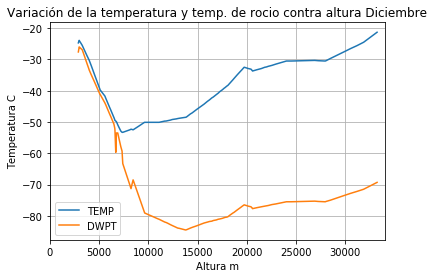
\includegraphics[scale=0.5]{grafica6.png}
\end{tabular}
\caption{Gráficas de variación de la temperatura y temperatura de rocio contra altura}

\end{figure}


\begin{figure}[h]
\begin{tabular}{ll}
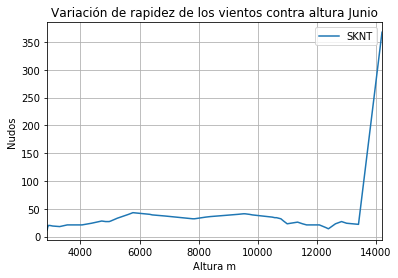
\includegraphics[scale=0.5]{grafica7.png}
&
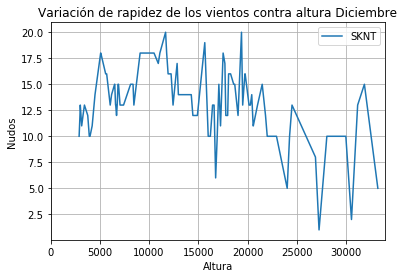
\includegraphics[scale=0.5]{grafica8.png}
\end{tabular}
\caption{Gráficas de variación de la rápidez de los vientos contra altura}

\end{figure}


\begin{figure}[h]
\begin{tabular}{ll}
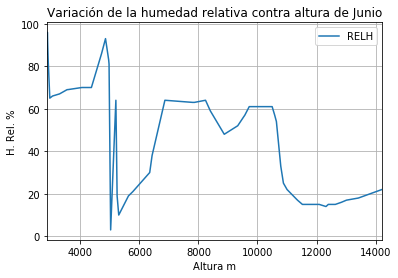
\includegraphics[scale=0.5]{grafica9.png}
&
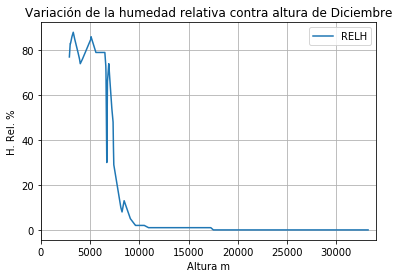
\includegraphics[scale=0.5]{grafica10.png}
\end{tabular}
\caption{Gráficas de variación de la humedad relativa contra altura}

\end{figure}


\section*{Conclusión}

A través de las herramientas modernas como Python en un entorno de programación intuitivo, además de la accesibilidad de datos, resulta muy fácil hacer un análisis de una gran cantidad de datos y obtener información de manera rápida. En este caso aprendimos como se comportan variables principales que describen el clima de una zona, comparando meses de invierno y verano.


\section*{Apéndice}


\begin{itemize}
\item     ¿Cuál es tu opinión general de esta actividad?

Fue muy útil un pŕimer acercamiento a leer datos reales y analizarlos a través de la nueva herramienta

\item     ¿Qué fue lo que más te agradó? ¿Lo que menos te agradó?

Me agradó la idea de comparar los datos meteorológicos del mismo lugar pero en diferente época del año. Lo que menos me agradó fue acomodar los datos para que sean legibles para el programa, pero es algo necesario que aprender.  

\item     ¿Qué consideras que aprendiste en esta actividad? 

Manejar datos en Python

\item     ¿Qué le faltó? ¿O le sobró?

Siento que se pudo agregar introducir algo nuevo que no se haya visto la actividad pasada

\item     ¿Qué mejoras sugieres a la actividad?
Me parece bien como es, tal vez comparar el procedimiento de la misma tarea pero con Fortran.

\end{itemize}

\section*{Bibliografía}

\begin{verbatim}
(2017). Numerical weather prediction. 12 de febrero 2018, de Wikipedia Sitio web: 
https://en.wikipedia.org/wiki/Numerical_weather_prediction

(2017). Atmospheric sounding. 12 de febrero 2018, de Wikipedia Sitio web:
https://en.wikipedia.org/wiki/Atmospheric_sounding

(2018). Weather balloon. 12 de febrero 2018, de Wikipedia Sitio web: 
https://en.wikipedia.org/wiki/Weather_balloon

(2018). Sondeos atmosféricos. 8 de febrero, 2018, de Universidad de Wyoming Sitio web:
http://weather.uwyo.edu/upperair/sounding.html
\end{verbatim}

\end{document}